\section{Methodology}
Most of the time, different business have unique data characteristics. To build a recommender system, especially, require customized algorithm for model tuning.  Having a sound business domain knowledge is very helpful in better using its data, creating the performant prediction model. In this paper, we propose a framework MVRec (meta-path embedding based Recommendation) that allow recommendation models to learn item features embedding by adapting custom domain knowledge in a generic way. 

\begin{figure*}[!t]
    \centering
    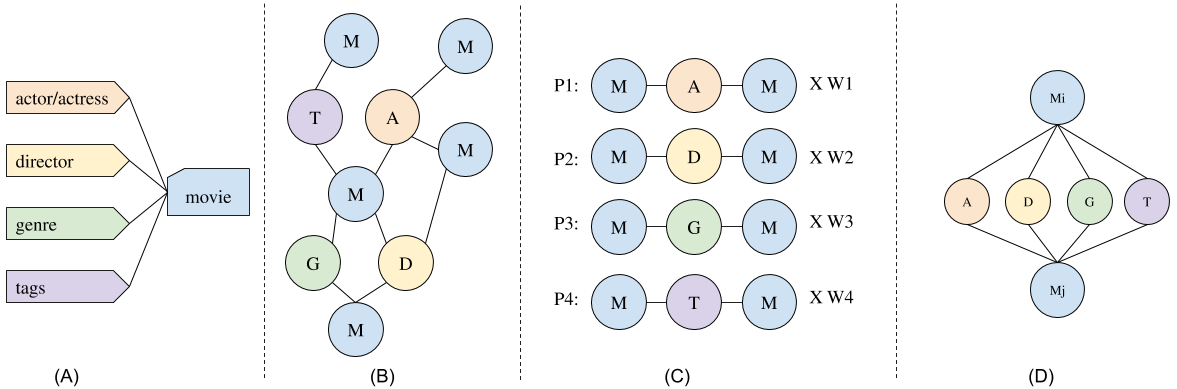
\includegraphics[width=0.8\textwidth]{figs/fig1.png}
    \caption{heterogeneous information graph based on item features}\label{fig:fe-graph}
\end{figure*}

One of the key idea of our approaches is inspired by recent research on graph-based embedding (reference) Instead of using random walk to learn low-dimensional item feature presentation, our approach introducing a pre-defined set of meta-path to create user interfered bias to control the walk random process from one node to another in HIN. The benefit of such practice can be review from 2 different fronts: 

\begin{enumerate}
    \item Intuitively, introducing user-defined sets of meta-path, allows the model to accommodate user background knowledge into the random walk process. This can prevent over-fitting on some common nodes that overcrowded by connections. i.e. comedy is the top genre in movie-lens data sets. Over 20 \% of the movie are comedies. However, most of the time user would not choose a movie purely based on genre alone.
    \item Categorical data is common but tricky to adapt into model learning. A common practice of handling categorical data is using one-hot (reference) encoding. However, it can quickly become a problem, when the categorical data has a lot of unique values. For example, the movie-lens dataset X actors, Y directors, X genre and so on. Using one-hot encoding normally leads to super large matrix size and high data sparsity.
\end{enumerate}

Consequently, as the item embedding is learned based on item features rather than depending on user-item interactions. This allows model to handle cold start problem and data sparsity problem effectively. 

\subsection{Problems and Definitions}\label{3PD}
Following definitions are used for describe our approach MVRec.

\begin{definition}[Heterogeneous Information Graph]
A information graph is $G = (V,E)$, where $V$ is the set of nodes (or entities) of the graph. $E$ is the set of edges connecting the nodes in $V$, $E \subset V \times V$. \newline
Two mapping functions: Entity type mapping function $\phi$: $V \rightarrow A$, and link type mapping function $\varphi$: $E \rightarrow R$, where $A$ and $R$ denote the sets of predefined entity and link types, and $|A| > 1$ or $|R| > 1$ indicating that there are more than one type.
\end{definition}

For example, we use movie attribute information to enrich user-item ratings in Movielens data set using graph model as shown in Fig. %\ref{fig:enrich}
In this paper we use \textit{``actors'', ``director'', ``writer'', ``genre''} etc. as different types of nodes. These nodes are in the same graph of user nodes and item nodes. How to process with different nodes in one graph? Graph schema indicates how different types of entities link with each other. It serves as a template to describe the structure as well as the semantic relationship between object types.

Between two entities $x$ and $y$, there are different paths connecting the two nodes. As for the case of Movielens, \textit{MovieA} and \textit{MovieB} can be connected via \textit{MovieA-Actor-MovieB} or \textit{MovieA-Director-MovieB} or \textit{MovieA-User-MovieB} path connections. We call those path, which containing multiple entities, Meta-Path.

\begin{definition}[Meta-Path]\label{def:metaPath}
A Meta-Path $\mathcal{P}$ is a path defined on the  graph schema $T_G = (A, R)$. \newline
Meta-Path $\mathcal{P}$ is denoted as $A_1 \xrightarrow{\text{r1}} A_2 \xrightarrow{\text{r2}} ... \xrightarrow{\text{rn}} A_n$. 

Relationship $R$ is denoted as $r1 \bullet r2 \bullet ... rn$ for different types of relationship between different types of entity nodes, where $\bullet $ denotes composition operator or relations.
\end{definition}

For Meta-Path $\mathcal{P}_i$ shares same graph schema, there could also be multiple path $p$ connecting source entity $a_i$ to target ${a}_{i+1}$. Each path $p$ inside Meta-Path $\mathcal{P}_i$ is a path instance, $p \in \mathcal{P}_i$. The number of path instances $p$ between $a_i$ and $\bm{a}_\text{i+1}$, is called path count. Reverse Meta-Path $\mathcal{P}^{'}$ is the reversed relation sequence of $\mathcal{P}_i$, if $\mathcal{P}^{'}$ is the reverse path of $\mathcal{P}$ in $T_G = (A, R)$, reverse path is denoted as $\mathcal{P}^\text{-1}$. \newline

Meta-Path $\mathcal{P}_1: A_1 \xrightarrow{r_1} A_2$ is the Meta-Path connects source entity type $A_1$ and target $A_2$.
Similarly, $\mathcal{P}_2: A_2 \xrightarrow{r_2} A_3$, $\mathcal{P}_2$ is the Meta-Path between source entity type $A_\text{2}$ and target entity type $A_\text{3}$.
Here we call $\mathcal{P}_1$ and $\mathcal{P}_2$ are contactable. Then $\mathcal{P}_1$ and $\mathcal{P}_2$ can be combined as $\mathcal{P}_{1,2}: A_1 \xrightarrow{r_1} A_2 \xrightarrow{r_2} A_3$. For example, $Movie \rightarrow Director$ and $Director \rightarrow Movie$ can be combined to $Movie \rightarrow Director \leftarrow Movie$. 

\subsection{Meta-path Based Random Walk}\label{3MF}

For items such as movies, books, music, there are a number of factors impacting users' decision. 

Instead of taking the one-hot encoding approach, treating each category value as a feature column. We propose to treat each feature category as an independent node type. Putting different feature type nodes and items together, here we formed a heterogeneous information graph. 

Next, we define sets of meta-path that is known to be effective factors for item-item similarities, based on the expert domain knowledge or based on feature analysis, such as, PCA for computation reduction purposes. For example, movie choice is closely linked to directors and its casts. Thus $Movie \rightarrow Director \leftarrow Movie$, $Movie \rightarrow Actor/Actress \leftarrow Movie$  can be very important meta-path in deciding how similar 2 movies are. We use those insights as a guideline to from a heterogeneous information graph based on item features. As shown in Fig. \ref{fig:fe-graph}

Each meta-path can derive a item-item similarity matrix $\mathbb{R}_i(\mathcal{P}_i)$, each different meta-path can be regarded as bias toward different feature aspects, so items co-occurrence can be learned separately under different meta-path.
as a result, item-item similarity score can be calculated by normalized meta-path similarity times meta-path weight.

\begin{equation}\label{itemsim}
    \mathcal{S}(v_i,v_j) = 
    \begin{cases}
         \sum\limits_{\substack{n=1}}^{n} \mathcal{R}_ij(\mathcal{P}_n,{W_n}),& \text{if } (v_{i}, .., v_{j}) \in \mathcal{P} \\
         0,              & \text{otherwise}
     \end{cases}
\end{equation}

$\mathcal{S}(v_i,v_j)$ stands for similarity between items $v_i$ and $v_j$ which shares the same node type. $R_ij()$ is a similarity function, where $\mathcal{P}_n, {W_n}$ stands for individual meta-path and its weights respectively. This end result provides guidance for the random walkers on our heterogeneous graph of item features. $(v_{i}, .., v_{j})$ is denoted as a meta-path instance, where $v_i$ is the starting node and $v_j$ the end node.

Given a heterogeneous graph $G = (V,E)$, and a meta-path set $[\mathcal{P}_1, \mathcal{P}_2, ... \mathcal{P}_n]$, the probability of transition is defined as following:

\begin{equation}\label{hetewalker}
    P(v_{i+1},\mathcal{P},w)= 
        \begin{cases}
            p({N^{t+1}(v_{i}^t)}),& \text{if } (v_{i+1}, .., v_{i}^t) \in \mathcal{P} \\
            0,              & \text{otherwise}
        \end{cases}
\end{equation}

$t$ is denoted as $t^th$ steps, as the walker traversing through the graph.
$p({N^{t+1}(v_{i}^t)})$ is a $softmax$ function on top of the neighbors of node $v_{i}^t$. 
that is:

\begin{equation}\label{softmaxwalker}
    p({N^{t+1}(v_{i}^t)}) = \frac{Exp(\mathcal{S}(v_i,v_j))}{\sum\limits_{\substack{n=1}}^{n} {Exp(\mathcal{S}(v_i,v_j)})}
\end{equation}

we enable skip-gram to learn the presentation of given node $v$:

\begin{equation}\label{skipgram}
    arg max
    \sum\limits_{\substack{v \in V}}
    \sum\limits_{\substack{c \in N(v)}}
    log p({c|v;\theta})
\end{equation}

$log p({c|v;\theta}))$ is the softmax function as defined in \cite{mikolov2013distributed} \cite{mikolov2013efficient}. In our approach, we substitute $log p({c|v;\theta}))$ with softmax function defined in equation \ref{softmaxwalker}. $c$ is denoted as $context$, in graph structure setting, $c$ is the neighboring nodes of given node $v$, i.e. $N(v)$. 

Finally, we introduce 3 hyper parameters to learn the item vector representation. $d$ for dimension size, $x$ for number of walks, and $l$ for depth of each random walk. 


\subsection{Pure Cold Start: MVRec-PCC}\label{3PCC}
One of common real world recommendation scenario is recommending new item to potential audiences/customers. For example, product launch, movie premier. Listings portal, such as, job listings (e.g. LinkedIn) and real estate listings (Zillow) faces constant pure cold start problem, where historical user-item interaction is not available to learn. 

In order to solve pure cold start problem, commonly feature based (content based) are one of limited way to make recommendation. 
Additionally, we adopt Pearson Correlation Coefficient (PCC) to be in combination with MVRec through the recommendation process. 
PCC is a popular measurement approach as defined in equation \ref{pcc}, unlike Cosine Similarity, PCC takes the difference of mean and variance between users' rating scale into account.

\begin{strip}
    \begin{equation}\label{pcc}
        S_{u_i,u_j}^{PCC} = 
        \dfrac{
            \sum_{v \in V_{u_i} \cap V_{u_j}} (r_{u_i,v}-\overline{r_{u_i}}) 
            * 
            (r_{u_j,v} - \overline{r_{u_j}})
        }
        {
            \sqrt{\sum_{v \in V_{u_i} \cap V_{u_j}} (r_{u_i,v}-\overline{r_{u_i}})^2} 
            * 
            \sqrt{\sum_{v \in V_{u_i} \cap V_{u_j}} (r_{u_j,v}-\overline{r_{u_j}})^2}
        }
    \end{equation}
\end{strip}

accordingly, we can normalized the user-item rating based on normalized user rating $\overline{u}$ overall:
\begin{equation}\label{pcc}
    NS(r_{u_i,v_j}) =  S_{u_i,\overline{u}}^{PCC}
\end{equation}

Consequently, we get the top ranked user by calculating as following:

\begin{algorithm}
    \caption{ranked users list}
    \begin{algorithmic}[1] 
    \REQUIRE~~\\ %Input
    New Item: $v$\\
    Existing user item ratings: ${R_{mxn}}$\\
    Items vectors: $\mathcal{V}$\\
    Top X nearest items: $X$\\
    Top K ranked users list rank: $K$\\
    \ENSURE~~\\ %Output
    \STATE Compute nearest items $TopN(v,\mathcal{V})$ based on $\mathcal{V}$ and $v$
    \STATE \textbf{for} x=1 : X
    \STATE \quad Compute normalized rating per user of $v_x$
    \STATE \quad Ranked users $RankedList(v_x) \leftarrow (u_i, NS(r_{u_i,v_x}))$
    \STATE \quad $TopKList(v) \leftarrow$ Top $K$ (user,rating) in $RankedList(v_x)$
    \STATE $RankedList(v)$ = \textbf{from} $TopKList(v)$ \textbf{group by} user \textbf{select} (user,$\sum{rating}$) \textbf{order by} $\sum{rating}$
    \RETURN Top K of $RankedList(v)$
    \end{algorithmic}\label{alg:1}
\end{algorithm}

In Section \ref{4_experiment}, we would show more detailed comparison results with traditional categorical one-hot encoding approach

\subsection{Sparse Recommendation: MVRec-BPR}\label{3BPR}
One of the other common cold start problem, that we commonly facing is sparse data. Matrix Factorization or CF based approach, try to learn user and item presentation (i.e. $U, V$) in a latent space jointly, normally suffers from data sparsity problem.


Here we propose, instead of learning $U, V$ jointly, we replace $V$ with meta-path based vectors $Vec(v)$. This approach provides several benefits:
\begin{enumerate}
        \item Reducing learning complexities
        \item Taking both item features and user-item interactions into account
        \item $Vec(v)$ is less impacted when user-item interactions are sparse 
\end{enumerate}

We use BPR as our optimization objective:

\begin{equation}\label{skipgram}
    arg max (u_i \cdot Vec(v)-u_j \cdot Vec(v)) - \dfrac{\lambda}{2}tr(U^TU)
\end{equation}


Based on the experiment result in Section \ref{4_experiment}, we see MVRec out performs widely used CF+ BPR by a large margin in sparse dataset. It also gained equivalent or minor advantage when the dataset is less sparse in non-cold start settings.


